%
% latex-sample.tex
%
% This LaTeX source file provides a template for a typical research paper.
%

%
% Use the standard article template.
%
\documentclass{article}

% The geometry package allows for easy page formatting.
\usepackage{geometry}
\geometry{letterpaper}

% Load up special logo commands.
\usepackage{doc}

% Package for formatting URLs.
\usepackage{url}

% Packages and definitions for graphics files.
\usepackage{graphicx}
\usepackage{epstopdf}
\DeclareGraphicsRule{.tif}{png}{.png}{`convert #1 `dirname #1`/`basename #1 .tif`.png}

%
% Set the title, author, and date.
%
\title{Interim Report of "Hadoop YARN Cloud Configuration Tool"}
\author{Group 9: Shiqian Xu, Jiang Gu, Pengyu Li, Liang Dong}
\date{}

%
% The document proper.
%
\begin{document}

% Add the title section.
\maketitle

% Add an abstract.
\section{Abstract}
 It is a tedious and painstaking to deploy a Hadoop cluster and debug a complex job.  Monitoring a Hadoop cluster is a large part of what a Hadoop developer does. Although third-party monitoring tools are available to monitor Hadoop,  We want to build our system from low-level APIs and compare various techniques used to monitor Hadoop cluster. Besides, we want to integrate our monitoring tool with AWS and docker. After all,  our project is aim to develop a tool to provide easy deployment and a real-time monitoring system of Hadoop YARN clusters on  cloud service provider. As workload changes, the system allows cluster to add or remove nodes on the fly. 		
\subsection{Overview}
According to the following Fig.1, the project mainly consists of CLI, monitor and scale. Main functionalities of this Command Line Interface(CLI) is to interact with AWS EC2 instances and Hadoop YARN Cluster Nodes.
\begin{figure}[h!]
 \centering
  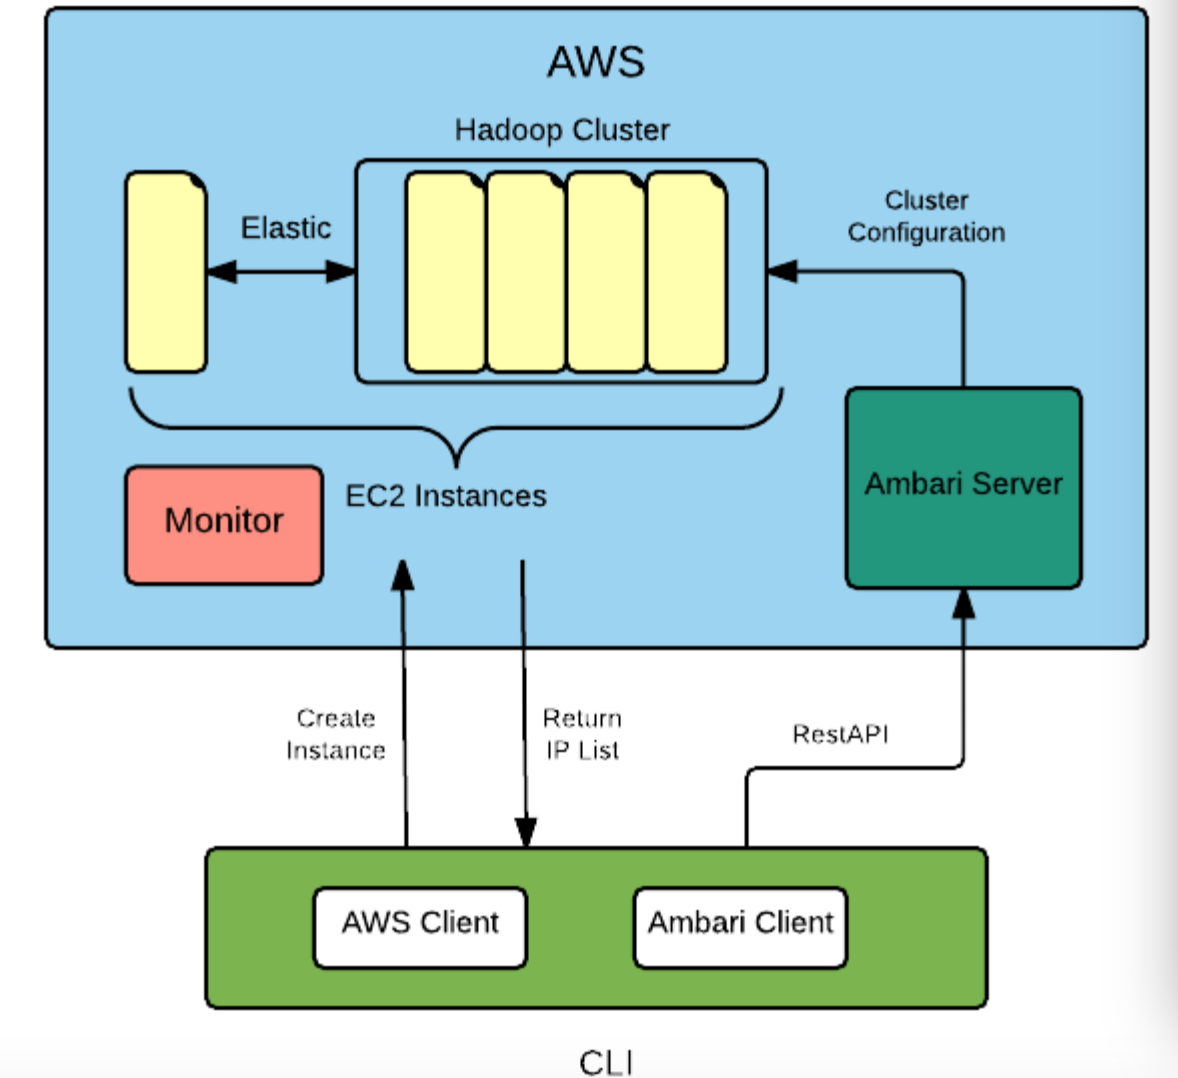
\includegraphics[width=0.5\textwidth,natwidth=700,natheight=500]{fig1.png}
 \caption{Fig. 1 Architecture of Hadoop project}
 \end{figure}
 The first part is CLI, we need to develop a CLI tool with many ease-use commands, which can interact with AWS, create EC2 instances, call Ambari Server commands to automatically deploy Hadoop Clusters on cloud foundry.
\begin{figure}[h!]
 \centering
  \includegraphics[width=0.5\textwidth,natwidth=700,natheight=200]{fig2.png}
 \caption{Fig. 2 Monitor Structure}
 \end{figure}
The second part is monitor, we will develop monitor client and server(See Fig.2). The monitor client can be deployed to each node of Hadoop cluster and AWS instances. They periodically send monitoring data back to monitor server. Monitor server will put together all clients data, store data into local log file.
The third part is scale, we will use Ambari Server to increase or decrease the cluster capacity, this behavior will be triggered by the utility ratio of cluster resource. One simple policy is to enforce a guaranteed cluster capacity requests (e.g. 75\% of the cluster resource) without some nodes being much more or less than other nodes utilized.


%
% Body text.
%
\section{Justification}

Our initial goal is to make Hadoop YARN cluster management easier because Hadoop cluster management is tedious. Using Apache Ambari, we are able to easily deploy the Hadoop Cluster. However, Ambari deployment only happens on local environment which works well with vagrant and VMs. As it is a trend to go on cloud, we decide to provide an intuitive, easy-to-use CLI combining AWS and Ambari interface to deploy Hadoop YARN on the cloud.

Beside, Apache Ambari only provides overview of the YARN cluster as a whole, which is not enough to satisfy all of our needs for this project. When we need to make a decision about adjustment to the cluster, the monitoring system should satisfy the following needs. First is flexible, not only a small cluster with a few nodes, it should be able to monitor thousands of node without much more extra resource assumption. Secondly, we are expecting to have a good understanding of the overview of the cluster  health and a deeper analysis of individual hadoop daemon performance along with traditional system resources(cpu, memory, io and network).  Additionally, to dynamically adjust the cluster nodes, we have to use the gathered data which should be stored in data warehouse.  Other modules should also easily access these data for analysis via a query interface. Base on these needs, we have to integrate current monitoring solution to provide more detailed monitor system to a YARN cluster(running in Docker containers) deployment.

We also consider that a cluster should be elastic, which should be able to increase or decrease  the cluster capacity dynamically. By adding/removing nodes, the cluster throughput could be increased or decreased based on the cluster load and scheduled applications. Based on previous step by setting up a monitoring system, we are expecting maintain a well-balanced cluster to ensure healthy and operational using these data. One simple policy is to enforce a guaranteed cluster capacity requests (e.g. 75\% of the cluster resource) without some nodes being much more or less than other nodes utilized.

The project is good practice for us to learn data intensive computing. AWS, Docker and other software represent the trend of software development. The project will lead us to investigate AWS API, docker deployment and distributed computing. At last, we will run some test cases to evaluate the performance of our implementation. Although the project is aimed at making the deployment and monitoring of Hadoop cluster easier, we are wondering if the management overhead will reduce the performance of the system. It will help us  get a better understanding about how to design the architecture for data intensive computing.



\section{Project Management}
\subsection{Goal}

Our team will develop a CLI to automatically deploy Hadoop clusters, real-time monitor  Hadoop YARN clusters and AWS instances, and scale clusters based on monitoring data.

\subsection{Milestones}
Most of our tasks involves pair programming. As a group of four, we separated into two pairs, working on the following tasks.\\
\textbf{Milestone 1: Finish CLI and basic module -- 3 week (group of 2 pairs on each task.)}\\
In the first phase of the project, most of us are involved with building small modules of the infrastructure, such as the CLI or the Ambari interfaces. During milestone1, we decide to finish the basic functionality of the CLI. We are able to use CLI to create cluster of instances in AWS and fetch the basic info such as IP address or security group, region information from AWS. Docker dependencies and Ambari should also be installed on each AWS node during this phase.\\
\emph{\textbf{Pair 1:}}\\
What:basic AWS function module such as instance creation and fetching instance info\\
Dependency: AWS SDK\\
Duration: 1 week\\
What:Prepare docker environment and run docker images in all instances\\
Dependency: Create instances with specified configuration.\\
Duration: 1-2 week\\
\emph{\textbf{Pair 2}}\\
What: Setup Ambari Server in one instance and create local Ambari client class\\
Dependency:  Apache Ambari\\
Duration: 1 week\\
What: Configure the hadoop cluster using Ambari client by REST API and Successfully run on cloud.\\
Dependencies: create local Ambari client class, Cloud Docker environment\\
Duration: 1-2week\\
\\
\emph{\textbf{Milestone 2: Monitor process of the Hadoop Cluster -- 4 to 5 weeks)}}\\
During Milestone 2, we will spend most of time on monitoring of Hadoop YARN cluster. To avoid adding any monitoring component to a hadoop docker image, we will isolate the monitor client into a different docker container on each AWS instances to collect data from Hadoop YARN metrics inside the running hadoop container. To be extensible to other cloud platform in the future, we should avoid directly using AWS API to get status on AWS machine by individual module to collect machine information. After gathering the data, the container will send the data to a centralized monitor nodes to process, store or further visualization data, where auto-scaling module will send request to fetch the data.  And then we will run some sample jobs to try with feature.\\
\emph{\textbf{Pair 1:}}\\
What: Deploy containers to monitor Hadoop YARN nodes\\
Dependencies: Hadoop YARN metrics\\
Duration: 1-2 week\\
\emph{\textbf{Pair 2:}}\\
What: Deploy containers to monitor AWS instances\\
Dependencies: AWS EC2 API,third party script\\
Duration: 1 week\\
\emph{\textbf{Whole Group}}\\
What: Build centralized server to get real-time monitor data from the distributed containers on each AWS node.\\
Dependencies: Hadoop YARN metrics\\
Duration: 2 week\\
What: Collect and store the data from Hadoop daemon and instances\\
Dependencies: Run test Hadoop jobs and able to monitor performance of cluster\\
Duration: 1 weeks\\
\emph{\textbf{Milestone 3: Autoscale Hadoop Cluster(potential)}}\\
The complexity of milestone 3 is depending on our progress.  To achieve the third milestone, we will investigate the strategies to add and remove instances based the on monitoring the Hadoop Cluster.\\
What: Add and Remove instances of Hadoop Cluster based on monitoring system  Dependency:  Collect and store the monitoring data from Hadoop daemon and instances  Duration: 2 weeks





\section{Verification}

The tool should be able to create instances on Amazon EC2 according to user input in the CLI. Create Hadoop clusters on those instances and providing a UI monitoring interface for user to inspect on status of Hadoop clusters.  Nodes will be auto added and deleted according to the running status of the cluster to make sure the system is in a stable state.


\section{Resources}
AWS

\section{Background}
Our application will integrate Hadoop provisioning and monitoring capabilities with the Ambari Rest API. Monitoring long and complex Hadoop jobs can be challenging[3]. It is also the focus of our project. The Ambari project is aimed at making Hadoop management simpler by developing software for provisioning, managing, and monitoring Apache Hadoop clusters[1]. Ambari provides an intuitive, easy-to-use Hadoop management web UI backed by its RESTful APIs.

We will use EC2 to test our implementation. Amazon Web Services (AWS), a collection of remote computing services, also called web services, make up a cloud-computing platform offered by Amazon.com. Amazon Elastic Compute Cloud(EC2) allows users to rent virtual computers on which to run their own computer applications.

We will deploy hadoop cluster on docker. Docker is an open platform for developers and sysadmins to build, ship, and run distributed applications[2]. Consisting of Docker Engine, a portable, lightweight runtime and packaging tool, and Docker Hub, a cloud service for sharing applications and automating workflows, Docker enables apps to be quickly assembled from components and eliminates the friction between development, QA, and production environments. As a result, IT can ship faster and run the same app, unchanged, on laptops, data center VMs, and any cloud.

% Generate the bibliography.
\begin{thebibliography}{2}

\bibitem{Ambari}
Apache Ambari Introduction: https://ambari.apache.org


\bibitem{Docker}
Docker Introduction: https://github.com/docker/docker



\bibitem{Wadkar}
Wadkar, Sameer, and Madhu Siddalingaiah
\newblock Monitoring Hadoop.
\newblock  Pro Apache Hadoop. Apress, 2014. 203-215.





\end{thebibliography}


\end{document}
